\section{Label Characteristics}

\subsection{Grouping Strategy}

Given the dataset's nature involving speech commands, effective grouping of the labels is crucial for both practical application and computational efficiency. Here’s a suggested approach for grouping:

\subsubsection{Methodology:}

\begin{itemize}
    \item \textbf{Semantic Similarity}: Group words based on their semantic meaning and usage in common speech scenarios. For example, commands like "an" and "aus" could be grouped under a category like "Commands."
\end{itemize}

\subsubsection{Proposed Groups:}

\begin{itemize}
    \item \textbf{Devices}: Includes "Fernseher", "Radio", "Licht" and "Alarm".
    \item \textbf{Appliances}: Includes "Heizung", "Lüftung", "Ofen" and "Staubsauger".
    \item \textbf{Commands}: Includes "an" and "aus".
    \item \textbf{Status}: Includes "warm", "offen".
    \item \textbf{Objects}: Includes "Leitung", "Spiegel", "Brötchen", "Haus" and "Schraube".
    \item \textbf{Miscellaneous}: All remaining words that do not neatly fit into the above categories but are still relevant for broad command recognition. Here includes "kann", "nicht", "wunderbar" and "other".
\end{itemize}

\subsection{Class Balance Assessment}

Class balance is critical in training machine learning models to prevent biases toward more frequent classes.

\subsubsection{Methodology:}

\begin{enumerate}
    \item \textbf{Quantitative Analysis}: Calculate the variance of each class in the dataset. Use bar charts to visually represent these distributions to quickly identify any imbalance.
    \item \textbf{Assess Impact}: Discuss how the imbalance might affect model training, particularly if some classes are underrepresented, potentially leading to poorer model performance on these classes.
\end{enumerate}

\subsubsection{Findings:}

\begin{itemize}
    \item \textbf{Imbalance Details}: The bar chart used to visualize these groups shows a noticeable imbalance between them. Especially Status and Commands are underrepresented. An obvious indicator of this imbalance is the Coefficient of Variance, which comes out to be 38\%.
    \item \textbf{Strategies for Mitigation}: Data augmentation or collecting more data, especially for the minority classes are potential approaches to balance the classes to improve model performance.
\end{itemize}

\begin{figure}[!ht]
	\centering
	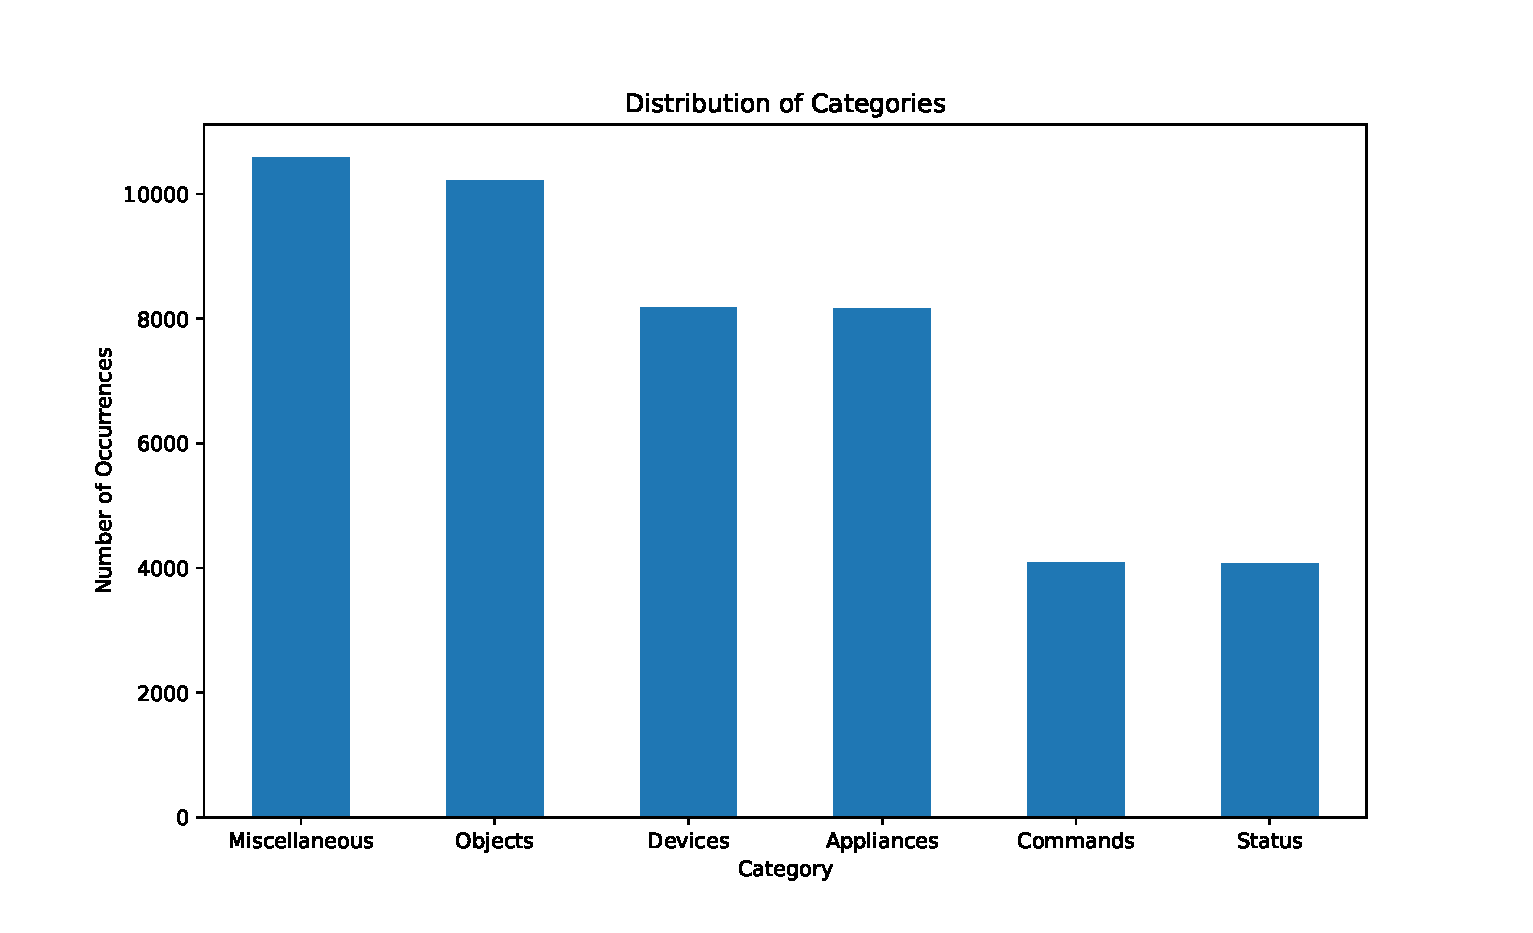
\includegraphics[scale=0.3]{fig/categories_dist}
	\vspace{-0.3cm}
	\caption{Categories Distribution.}
	\label{fig:CategoriesDistribution}
	\vspace{-0.1cm}
\end{figure}